\documentclass[11pt,a4paper]{article}
\usepackage[margin=23mm,headheight=15pt]{geometry}
\usepackage[T1]{fontenc}
\usepackage[utf8]{inputenc}
\usepackage{lmodern}
\usepackage{microtype}
\usepackage{amsmath,amssymb,amsfonts,mathtools,bm}
\usepackage{booktabs,tabularx,array,longtable,multicol}
\usepackage[dvipsnames,table]{xcolor}
\usepackage{tikz}
\usetikzlibrary{arrows.meta,positioning,fit,calc,shapes.geometric}
\usepackage[most]{tcolorbox}
\usepackage{listings}
\usepackage{fancyhdr}
\usepackage{hyperref}
\usepackage[nameinlink,noabbrev]{cleveref}
\usepackage{enumitem}
\usepackage{caption}
\setlist[itemize]{itemsep=3pt,topsep=4pt}
\definecolor{navy}{HTML}{193C5B}
\definecolor{blue}{HTML}{24689A}
\definecolor{teal}{HTML}{18786E}
\definecolor{warm}{HTML}{A15C31}
\definecolor{lightblue}{HTML}{EFF6FA}
\definecolor{lightgray}{HTML}{F5F7F8}
\hypersetup{colorlinks=true,linkcolor=navy,urlcolor=blue,citecolor=teal,pdftitle={Finite-Strain FFT: Detailed Notes Through Equation 24},pdfauthor={Technical study notes based on de Geus et al. (2017)}}
\pagestyle{fancy}
\fancyhf{}
\fancyhead[L]{\small\color{navy}Finite-strain FFT: derivation and interpretation}
\fancyhead[R]{\small\color{navy}de Geus et al. (2017)}
\fancyfoot[C]{\thepage}
\renewcommand{\headrulewidth}{0.35pt}
\setcounter{tocdepth}{2}
\numberwithin{equation}{section}
\renewcommand*{\theHequation}{\theHsection.\number\inputlineno}
\newcommand{\F}{\mathbf F}
\newcommand{\Pstress}{\mathbf P}
\newcommand{\Gop}{\mathbb G}
\newcommand{\Kop}{\mathbb K}
\newcommand{\xvec}{\mathbf x}
\newcommand{\Xvec}{\mathbf X}
\newcommand{\uve}{\mathbf u}
\newcommand{\zero}{\mathbf0}
\newcommand{\avg}[1]{\langle #1\rangle}
\newcommand{\FT}{\mathcal F}
\newcommand{\IFFT}{\mathcal F^{-1}}
\newcommand{\diff}{\mathop{}\!\mathrm d}
\newcommand{\T}{^{\mathsf T}}
\newcommand{\paper}[1]{\tag{#1}}
\newcommand{\Dtag}[1]{\tag{D#1}}
\newtcolorbox{insight}[1][]{colback=lightblue,colframe=blue!55!white,boxrule=.55pt,arc=2mm,breakable,title={\bfseries Key interpretation},coltitle=navy,fonttitle=\small,#1}
\newtcolorbox{caution}[1][]{colback=warm!5,colframe=warm!65!white,boxrule=.55pt,arc=2mm,breakable,title={\bfseries Notation or implementation caution},coltitle=warm!70!black,fonttitle=\small,#1}
\newtcolorbox{worked}[1][]{colback=teal!4,colframe=teal!55!white,boxrule=.55pt,arc=2mm,breakable,title={\bfseries Worked interpretation},coltitle=teal!70!black,fonttitle=\small,#1}
\lstdefinestyle{code}{basicstyle=\ttfamily\footnotesize,backgroundcolor=\color{lightgray},frame=single,rulecolor=\color{blue!25},breaklines=true,columns=fullflexible,keywordstyle=\color{blue!80!black},commentstyle=\color{teal!80!black},showstringspaces=false,tabsize=3}
\lstset{style=code}
\tikzset{flow/.style={draw=blue!65!black,fill=lightblue,rounded corners=2pt,align=center,text width=10.0cm,minimum height=10mm,inner sep=5pt,font=\small},arr/.style={-Latex,thick,draw=blue!85!black},minor/.style={draw=teal!70!black,fill=teal!7,rounded corners=2pt,align=center,text width=10.0cm,minimum height=8mm,inner sep=4pt,font=\small}}

\begin{document}
\pagenumbering{roman}
\begin{titlepage}
\centering
\vspace*{1.4cm}
{\color{navy}\rule{\textwidth}{1.3pt}}\\[0.8cm]
{\Huge\bfseries Finite-Strain FFT-Based\\[0.17cm] Nonlinear Mechanics}\\[0.4cm]
{\LARGE A Detailed Derivation and Study Guide}\\[0.6cm]
{\large\bfseries Through Section 2, Equations (1)--(24),\\ with Appendix D explained}\\[1.0cm]
{\color{navy}\rule{\textwidth}{0.7pt}}\\[1.1cm]
\begin{minipage}{0.89\textwidth}
\large
\textbf{Based on:} T.~W.~J. de Geus, J. Vond\v{r}ejc, J. Zeman, R.~H.~J. Peerlings, and M.~G.~D. Geers, ``Finite strain FFT-based non-linear solvers made simple,'' \emph{Computer Methods in Applied Mechanics and Engineering}, \textbf{318} (2017), 412--430. DOI: \href{https://doi.org/10.1016/j.cma.2016.12.032}{10.1016/j.cma.2016.12.032}; \href{https://arxiv.org/abs/1603.08893}{arXiv:1603.08893v3}.
\end{minipage}
\vfill
\begin{tcolorbox}[colback=lightblue,colframe=blue!35!white,boxrule=.5pt,width=.93\textwidth]
\centering\large\bfseries Guiding idea\\[5pt]
\normalsize Local stress and consistent tangent at each voxel\\
$\Downarrow$\\
Global projected equilibrium through FFT\\
$\Downarrow$\\
Newton--Krylov solution without assembling a global stiffness matrix
\end{tcolorbox}
\vspace{1cm}
{\normalsize Technical notes prepared to consolidate the preceding discussions on FFT, DFT, convolution, Green operators, voxel discretization, projection, Newton--CG, and the paper's Appendix D.}\\[.5cm]
{\normalsize October 2026}
\end{titlepage}
\setcounter{page}{2}
\tableofcontents
\clearpage
\pagenumbering{arabic}

\section{Purpose, scope and notation}
These notes give a step-by-step explanation of the \textbf{entire mathematical development through Equation (24)} in Section 2 of de Geus et al.\ \cite{degeus2017}. They also summarize related explanations from the discussion: why a periodic voxel-based RVE is useful, convolution and the convolution theorem, FT versus DFT versus FFT, interpretation of the Fourier frequencies, a cuboidal cell, comparison with FEM, the distinction between local and global solution, the full Newton--CG nesting, and the proof of the projector in \textbf{Appendix D (Equations (50)--(55))}.

\textbf{Traceability convention.} Displayed equations explicitly tagged \textbf{(1)}--\textbf{(24)} and \textbf{(D50)}--\textbf{(D55)} identify equations corresponding to the source paper. Untagged displayed mathematics is added to unpack those steps. In the appendix, the original paper uses the numbers (50)--(55); the prefix D is added here only for clarity. Derivations and educational examples in this document are explanations, not claims of further results presented in the paper.

\subsection{Symbols and tensor contraction}
\begin{center}\small
\begin{tabularx}{\textwidth}{@{}lX@{}}\toprule
Symbol & Meaning\\\midrule
$\Omega_0$, $V$ & Undeformed periodic RVE and its volume.\\
$\Xvec$, $\xvec$ & Reference and current spatial coordinates.\\
$\F=\partial\xvec/\partial\Xvec$ & Deformation gradient, $F_{ij}=\partial x_i/\partial X_j$.\\
$\Pstress$ & First Piola--Kirchhoff stress, conjugate to $\F$.\\
$\bar\F$ & Prescribed macroscopic (volume-average) deformation gradient.\\
$\delta\F$ & Compatible virtual fluctuation or a Newton correction (context indicated).\\
$\delta\widetilde\F$ & Arbitrary periodic test tensor field, before projection.\\
$\Gop$, $\hat\Gop$ & Real-space compatibility projector and its Fourier representation.\\
$\Kop$, $\Kop^{LT}$ & Constitutive tangent and its paper-specific left-transposed arrangement.\\
$N_a(\Xvec)$ & Global trigonometric cardinal shape function for grid point $a$.\\
$\mathbf q=(q_x,q_y,q_z)$ & Integer Fourier mode (frequency-index) vector.\\
$\bm\xi=(q_x/L_x,q_y/L_y,q_z/L_z)$ & Cell-length-scaled frequency vector.\\
$\FT$, $\IFFT$ & Fourier transform and inverse; on grid samples, implemented by DFT/FFT.\\
$*$ & Spatial convolution; distinct from an ordinary tensor contraction.\\\bottomrule
\end{tabularx}
\end{center}
The source paper uses a \emph{transpose-aware} contraction convention: for two second-order tensors, $\mathbf A:\mathbf B=\sum_{ij} A_{ij}B_{ji}$. Thus $\delta\F:\Pstress^T=\sum_{ij}\delta F_{ij}P_{ij}$ is the usual virtual-work pairing. For intuitive index manipulations we also use the standard component convention $\delta P_{ij}=C_{ijkl}\delta F_{kl}$, and explicitly identify it as $C$ rather than silently equating it with the paper's ordered $K$. The left-transpose $LT$ in the paper means interchange of the \emph{first two indices} of the fourth-order tensor.

\section{Why an FFT solver? The mechanical problem and the FEM comparison}
\subsection{Periodic microstructures and homogenization}
A representative volume element (RVE) resolves grains, phases, inclusions, or orientation heterogeneity while representing a statistically homogeneous material at a larger scale. The source considers a \emph{periodic} RVE, one or more constitutive phases, and an imposed macroscopic deformation. The goal is the heterogeneous equilibrated field and its volume average.

The finite-strain kinematics can be written as
\[
\xvec(\Xvec)=\bar\F\Xvec+\widetilde\uve(\Xvec),\qquad
\F(\Xvec)=\bar\F+\nabla_0\widetilde\uve(\Xvec),\qquad
\avg{\nabla_0\widetilde\uve}=\zero.
\]
Here $\widetilde\uve$ is periodic, and $\bar\F=\avg{\F}$. Across opposite faces of the periodic cell, displacement fluctuations are paired; the corresponding equilibrium tractions cancel in the boundary part of virtual work. \textbf{The unknown local deformation field remains globally coupled.}

\subsection{Grid, nodal values and quadrature}
The RVE is sampled on a regular Cartesian grid. In the illustrative collocation convention of the paper's Fig.~1, each pixel/voxel has one computational node at its center, and the quadrature point coincides with that node. The material update uses local $\F_a\mapsto \Pstress_a,\Kop_a$. Unlike standard eight-node hexahedral FEM with Gauss points inside an element, there is not a separate set of FEM displacement nodes and integration points.

\begin{center}
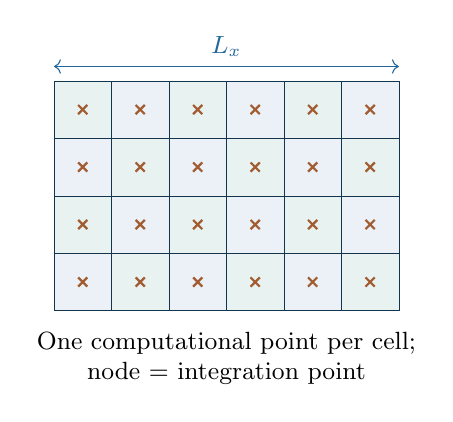
\begin{tikzpicture}[scale=.73]
  \foreach \i in {0,...,5}{\foreach \j in {0,...,3}{
    \pgfmathparse{mod(\i+\j,2)==0?"blue!9":"teal!10"}
    \fill[\pgfmathresult] (\i,\j) rectangle ++(1,1);
    \draw[blue!50!black,very thin] (\i,\j) rectangle ++(1,1);
    \draw[warm,thick] (\i+.42,\j+.42) -- (\i+.58,\j+.58) (\i+.42,\j+.58)--(\i+.58,\j+.42);
  }}
  \node[font=\small,anchor=north,align=center] at (3,-.2) {One computational point per cell;\\ node $=$ integration point};
  \draw[<->,blue] (0,4.25)--node[above,font=\small]{$L_x$}(6,4.25);
\end{tikzpicture}
\end{center}

In FEM, $\uve^e(\Xvec)=\sum_{a\in e}N_a^e(\Xvec)\uve_a$ uses piecewise-polynomial functions supported locally on one element or a small patch of elements. Here $\F(\Xvec)\approx\sum_{a=1}^{n}N_a(\Xvec)\F_a$ uses \emph{trigonometric polynomials with global support} across the periodic RVE. This is a statement about interpolation; \textbf{both FEM and FFT solve a global equilibrium problem}.

\subsection{Cuboidal RVEs are supported}
The geometry may be a cuboid, e.g. $L_x=L_y\neq L_z$. One can choose $N_x,N_y,N_z$ independently, with spacings $\Delta x=L_x/N_x$ etc. A cube is not necessary; the Fourier projector includes $1/L_i$ factors. A thin periodic box remains a three-dimensional mechanics model; reducing $L_z$ does not by itself impose plane stress or plane strain.

\section{Fourier and Green-operator background}
\subsection{Continuous Fourier transform, periodic Fourier series, DFT and FFT}
For an integrable continuous 1D field, using angular wave number $k$,
\[
\hat f(k)=\int_{-\infty}^{\infty}f(x)e^{-ikx}\diff x,
\qquad f(x)=\frac1{2\pi}\int_{-\infty}^{\infty}\hat f(k)e^{ikx}\diff k.
\]
For a periodic cell of length $L$, its harmonic expansion uses integer $q$ and $k_q=2\pi q/L$:
\[
f(x)=\sum_{q\in\mathbb Z}\hat f_q e^{i2\pi qx/L},\qquad
\hat f_q=\frac1L\int_0^L f(x)e^{-i2\pi qx/L}\diff x.
\]
For $N$ spatial samples $f_n=f(nL/N)$, the \emph{discrete Fourier transform} and inverse are
\[
F_m=\sum_{n=0}^{N-1}f_n e^{-i2\pi mn/N},\qquad
f_n=\frac1N\sum_{m=0}^{N-1}F_m e^{i2\pi mn/N}.
\]
\textbf{DFT} is the defined discrete mathematical transform. \textbf{FFT} is the family of fast algorithms that compute \emph{the same} DFT (modulo roundoff). A direct DFT needs roughly $O(N^2)$ operations, whereas a standard FFT requires $O(N\log N)$. A 3D FFT is formed by transforming along each coordinate direction. On finite periodic grids, convolution is circular and must use compatible FFT normalization and ordering.

\subsection{The convolution integral and why FFT turns it into multiplication}
For two functions,
\[
h(x)=(f*g)(x)=\int_{-\infty}^{\infty}f(x-y)g(y)\diff y.
\]
The variable $y$ identifies a source location and $f(x-y)$ weighs that location's contribution to the response at $x$. Transform the convolution:
\begin{align*}
\hat h(k)
&=\int_{-\infty}^{\infty}\!\!\left[\int_{-\infty}^{\infty}f(x-y)g(y)\diff y\right] e^{-ikx}\diff x\\
&=\int_{-\infty}^{\infty}g(y)\left[\int_{-\infty}^{\infty}f(x-y)e^{-ikx}\diff x\right]\diff y\\
&\overset{z=x-y}{=}\int g(y)\left[\int f(z)e^{-ik(z+y)}\diff z\right]\diff y\\
&=\underbrace{\int f(z)e^{-ikz}\diff z}_{\hat f(k)}
\underbrace{\int g(y)e^{-iky}\diff y}_{\hat g(k)}.
\end{align*}
Therefore the \emph{convolution theorem} reads
\[
\boxed{\FT\{f*g\}=\hat f\,\hat g.}
\]
The crucial identity is $e^{-ik(z+y)}=e^{-ikz}e^{-iky}$. For tensor fields, the product is replaced with the specified tensor contraction. For $N$ samples, circular convolution in physical space is evaluated via one FFT, pointwise multiplication, and an inverse FFT, instead of explicitly summing over every source location for every output point.

\subsection{Classical reference-medium Green operator versus the paper's projector}
In classical \emph{small-strain} periodic homogenization one can add/subtract a homogeneous reference stiffness $\mathbb C^0$:
\[
\bm\sigma(\Xvec)=\mathbb C(\Xvec):\bm\varepsilon(\Xvec)
=\mathbb C^0:\bm\varepsilon(\Xvec)+\bm\tau(\Xvec),\qquad
\bm\tau=(\mathbb C-\mathbb C^0):\bm\varepsilon.
\]
The polarization stress $\bm\tau$ acts as a source in the homogeneous reference problem. With its strain Green operator $\bm\Gamma^0$,
\[
\bm\varepsilon(\Xvec)=\bar{\bm\varepsilon}
-\int_{\Omega_0}\bm\Gamma^0(\Xvec-\mathbf Y):\bm\tau(\mathbf Y)\diff\mathbf Y.
\]
For nonzero Fourier modes this becomes $\hat{\bm\varepsilon}(\mathbf k)=-\hat{\bm\Gamma}^0(\mathbf k):\hat{\bm\tau}(\mathbf k)$. The \emph{reference Green operator} depends on $\mathbb C^0$; an unsuitable choice may affect convergence. The variational method in the source instead introduces a projector $\Gop$ based only on wavevector geometry. \textbf{The two operators are not identical}: one represents a chosen homogeneous reference mechanics problem; the other projects onto a kinematic compatible subspace.

\section{Section 2.1: Problem statement --- Equations (1)--(2)}
Consider a periodic RVE $\Omega_0$, possibly containing multiple material phases. In the absence of body forces, static equilibrium pulled back to the undeformed configuration is
\begin{equation}\nabla_0\cdot\Pstress^T=\zero.\paper{1}\label{p1}\end{equation}
In the authors' index convention, this means
\[
\frac{\partial P_{ij}}{\partial X_j}=0\quad(i=1,2,3),\qquad
\frac{\partial P_{11}}{\partial X_1}+\frac{\partial P_{12}}{\partial X_2}+\frac{\partial P_{13}}{\partial X_3}=0.
\]
The stress depends nonlinearly on the deformation gradient:
\begin{equation}\Pstress=\Pstress(\F).\paper{2}\label{p2}\end{equation}
The main derivation uses finite-strain \emph{nonlinear elasticity}; this is explicitly the simplifying assumption stated in the source. A history-dependent crystal plasticity extension has the more general trial-state form $\Pstress=\Pstress(\F,\bm\alpha)$, where $\bm\alpha$ contains internal variables, but this adds constitutive detail not required to derive Eqs. (1)--(24).

\begin{insight}
The goal is \emph{not} to solve an independent local equilibrium problem for every voxel: it is to find the field $\F(\Xvec)$ such that the constitutively evaluated stress satisfies the \emph{global} divergence equation and compatible periodic kinematics.
\end{insight}

\section{Section 2.2: Weak form --- Equations (3)--(5)}
\subsection{Multiply strong equilibrium by a virtual displacement}
Multiply Eq. (1) by an arbitrary admissible periodic virtual displacement $\delta\xvec$ and integrate:
\begin{equation}
\int_{\Omega_0}\delta\xvec\cdot(\nabla_0\cdot\Pstress^T)\diff\Omega_0=0.
\paper{3}\label{p3}\end{equation}
Index-wise this is $\int_{\Omega_0}\delta x_i\,\partial P_{ij}/\partial X_j\diff\Omega_0=0$.

\subsection{Integration by parts and cancellation of boundary contributions}
The product rule gives
\[
\frac{\partial}{\partial X_j}(\delta x_i P_{ij})
=\frac{\partial\delta x_i}{\partial X_j}P_{ij}
+\delta x_i\frac{\partial P_{ij}}{\partial X_j}.
\]
Integrating and invoking the divergence theorem,
\[
0=\underbrace{\int_{\partial\Omega_0}\delta x_i P_{ij}n_j\diff S}_{=0\text{ for periodic virtual fluctuations and opposite tractions}}
-\int_{\Omega_0}\frac{\partial\delta x_i}{\partial X_j}P_{ij}\diff\Omega_0.
\]
The remaining internal virtual-work statement is, in the \emph{paper's notation},
\begin{equation}
\int_{\Omega_0}\nabla_0\delta\xvec^T:\Pstress^T\diff\Omega_0=0.
\paper{4}\label{p4}\end{equation}
The physical content is $\int_{\Omega_0}(\partial\delta x_i/\partial X_j)P_{ij}\diff\Omega_0=0$. The transpose notation can be confusing unless the contraction convention is stated (see Section 1).

\subsection{Replace the virtual displacement gradient with a compatible virtual \texorpdfstring{$\F$}{F}}
Since $F_{ij}=\partial x_i/\partial X_j$, define $\delta F_{ij}=\partial\delta x_i/\partial X_j$. Then Eq. (4) becomes
\begin{equation}
\int_{\Omega_0}\delta\F:\Pstress^T\diff\Omega_0=0.
\paper{5}\label{p5}\end{equation}
\textbf{Crucial change from FEM:} in conventional displacement FEM, $\delta\F$ is formed from a compatible displacement interpolation. In the paper's FFT formulation, $\F$ is the primary nodal field; an arbitrary tensor assignment may \emph{not} be a displacement gradient. Compatibility must therefore be imposed independently.

For sufficiently smooth fields on a simply connected domain, a gradient field satisfies
\[
\frac{\partial F_{ij}}{\partial X_k}=\frac{\partial F_{ik}}{\partial X_j},\qquad\text{or row-wise }\nabla_0\times\F_{i\bullet}=\zero.
\]
Periodic gradient fluctuations must also have \emph{zero average}; constant mean deformation is prescribed separately. The projector introduced next enforces the appropriate zero-mean periodic gradient space.

\section{Section 2.3: Projecting the test functions --- Equations (6)--(7)}
The paper introduces a fourth-order kernel $\Gop$ that takes an arbitrary field $\widetilde{\mathbf A}$ to its compatible part:
\begin{equation}
\Gop*\widetilde{\mathbf A}=\mathbf A.
\paper{6}\label{p6}\end{equation}
The star denotes spatial convolution, not ordinary pointwise contraction. For the variation in Eq. (5), let $\delta\F=\Gop*\delta\widetilde\F$. Substitution gives
\begin{equation}
\begin{aligned}
\int_{\Omega_0}(\Gop*\delta\widetilde\F):\Pstress^T\diff\Omega_0
&=\int_{\Omega_0}\delta\widetilde\F:(\Gop*\Pstress)\diff\Omega_0\\[-1pt]
&=0.
\end{aligned}
\paper{7}\label{p7}\end{equation}
The second equality uses the self-adjoint/symmetric projection under the paper's tensor pairing. Equation (7) now holds for \emph{arbitrary periodic} test tensors $\delta\widetilde\F$; the compatibility restriction has been absorbed by the projection. This does \emph{not} mean every trial $\F$ is automatically compatible. Compatibility of the actual deformation-gradient field is handled through the admissible update subspace and Krylov iteration, as explained around Eq. (23).

\begin{insight}
For the test field, $\Gop$ converts an arbitrary virtual tensor into a compatible virtual gradient. For stress, the condition $\Gop:\Pstress=0$ says that the equilibrated stress is orthogonal to all compatible periodic virtual gradients. Stress itself need not be zero.
\end{insight}

\section{Section 2.4: Trigonometric Galerkin discretization --- Equations (8)--(12)}
\subsection{Trial and test expansions}
Let there be $n=N_xN_yN_z$ collocation nodes $\Xvec_a$. Use the same trigonometric cardinal basis $N_a(\Xvec)$ for the trial field and the arbitrary test field (Galerkin discretization):
\begin{equation}
\F(\Xvec)\simeq\sum_{a=1}^{n}N_a(\Xvec)\F_a=\mathbf N^T(\Xvec)\underline\F.
\paper{8}\label{p8}\end{equation}
\begin{equation}
\delta\widetilde\F(\Xvec)\simeq\sum_{a=1}^{n}N_a(\Xvec)\delta\widetilde\F_a
=\mathbf N^T(\Xvec)\delta\underline{\widetilde\F}.
\paper{9}\label{p9}\end{equation}
The underline indicates the column collecting tensor values over the grid, e.g.
\begin{equation}
\underline\F=\begin{bmatrix}\F_1&\F_2&\cdots&\F_n\end{bmatrix}^T.
\paper{10}\label{p10}\end{equation}
Unlike conventional FEM bases, trigonometric interpolation functions are globally supported throughout the periodic RVE, but are \emph{interpolatory}:
\begin{equation}
N_a(\Xvec_b)=\delta_{ab}.
\paper{11}\label{p11}\end{equation}
They additionally satisfy $\sum_{a=1}^{n}N_a(\Xvec)=1$ (partition of unity). At a grid point $b$, Eq. (8) therefore returns exactly $\F(\Xvec_b)=\F_b$. Global support refers to interpolation between grid points; it does not imply evaluating constitutive models at every other point.

\subsection{Derivation of Equation (12)}
Starting from Eq. (7), expand the test field:
\begin{align*}
0&=\int_{\Omega_0}\left[\sum_{a=1}^{n}N_a(\Xvec)\delta\widetilde\F_a\right]:(\Gop*\Pstress)(\Xvec)\diff\Omega_0\\
&=\sum_{a=1}^{n}\delta\widetilde\F_a:\underbrace{\int_{\Omega_0}N_a(\Xvec)(\Gop*\Pstress)(\Xvec)\diff\Omega_0}_{\text{nodal projected residual}}.
\end{align*}
The nodal test tensors are independent of $\Xvec$, so they can be taken outside the integral. In compact form this is
\begin{equation}
(\delta\underline{\widetilde\F})^T:\int_{\Omega_0}\mathbf N(\Gop*\Pstress)\diff\Omega_0=0.
\paper{12}\label{p12}\end{equation}
At this stage the weak form is discretized, but the global projected residual has not yet been converted to an efficient FFT computation.

\section{Section 2.5: Quadrature and Fourier projection --- Equations (13)--(20)}
\subsection{From arbitrary tests to discrete equilibrium (Eq. 13)}
Since Eq. (12) holds for every arbitrary nodal test value, the coefficient of each one must vanish:
\begin{equation}
\int_{\Omega_0}\mathbf N(\Gop*\Pstress)\diff\Omega_0=\underline{\mathbf O}.
\paper{13}\label{p13}\end{equation}
For a particular node $a$, this expresses $\int_{\Omega_0}N_a(\Gop*\Pstress)\diff\Omega_0=\zero$.

\subsection{Trapezoidal quadrature at collocation nodes (Eq. 14)}
The periodic uniform-grid trapezoidal quadrature assigns the same weight $V/n$ to each point:
\[
\int_{\Omega_0}h(\Xvec)\diff\Omega_0\simeq\frac{V}{n}\sum_{b=1}^{n}h(\Xvec_b).
\]
Dropping the common nonzero weight, the paper writes
\begin{equation}
\sum_{b=1}^{n}\mathbf N(\Xvec_b)[\Gop*\Pstress](\Xvec_b)=\underline{\mathbf O}.
\paper{14}\label{p14}\end{equation}
At node $a$, the cardinal property $N_a(\Xvec_b)=\delta_{ab}$ reduces this to $[\Gop*\Pstress](\Xvec_a)=\zero$: \emph{a projected residual tensor at each grid location}. The projection itself is still a global spatial operation.

\subsection{Convolution theorem gives the FFT implementation (Eq. 15)}
By Fourier transforming the stress field, applying the Fourier-space projector, and transforming back,
\begin{equation}
\IFFT\left\{\hat\Gop:\FT\{\Pstress\}\right\}=\underline{\mathbf O}.
\paper{15}\label{p15}\end{equation}
This involves: (i) forward DFT computed by FFT, (ii) a tensor contraction at every frequency, and (iii) inverse FFT. The paper abbreviates it as
\begin{equation}
\Gop:\underline\Pstress=\underline{\mathbf O},
\paper{16}\label{p16}\end{equation}
where $\Gop:\underline\Pstress$ denotes \emph{the complete FFT projection}, not just a pointwise double contraction between tensors in physical space.

\subsection{Local constitutive values (Eq. 17)}
The complete array of voxel stresses is
\begin{equation}
\underline\Pstress=\begin{bmatrix}
\Pstress_1(\F_1)&\Pstress_2(\F_2)&\cdots&\Pstress_n(\F_n)
\end{bmatrix}^T.
\paper{17}\label{p17}\end{equation}
Although $\Pstress_a(\F_a)$ is obtained locally, the operator in Eq. (16) includes the mechanical coupling among all voxels. There is one \emph{global} equilibrium solve, not $n$ independent equilibrium solves.

\subsection{Fourier-space block diagonal structure (Eq. 18)}
Because convolution is multiplication in frequency space, modes are not mixed \emph{by the projector alone}. The Fourier representation is diagonal \emph{in tensor blocks}:
\begin{equation}
\hat\Gop=\begin{bmatrix}
\hat\Gop(\mathbf q_1)&0&\cdots&0\\
0&\hat\Gop(\mathbf q_2)&\cdots&0\\
\vdots&\vdots&\ddots&\vdots\\
0&0&\cdots&\hat\Gop(\mathbf q_n)
\end{bmatrix}.
\paper{18}\label{p18}\end{equation}
Each diagonal entry is a \emph{fourth-order tensor} acting on a nine-component second-order tensor in 3D. In scalar-component form this is a block-diagonal $9n\times9n$ operator with $9\times9$ blocks, \emph{not} in general a scalar diagonal matrix. Each block corresponds to a Fourier mode, not to a physical voxel.

\subsection{Projection tensor and scaled spatial frequencies (Eq. 19)}
For the main-text discretization with odd grid counts, the authors give
\begin{equation}
\hat G_{ijlm}(\mathbf q)=
\begin{cases}
0,&\mathbf q=\zero,\\[5pt]
\displaystyle \frac{\delta_{im}\xi_j(\mathbf q)\xi_l(\mathbf q)}{\bm\xi(\mathbf q)\cdot\bm\xi(\mathbf q)},&\mathbf q\ne\zero,
\end{cases}
\quad
\xi_i(\mathbf q)=\frac{q_i}{L_i}.
\paper{19}\label{p19}\end{equation}
The integer spatial-frequency index $q_i$ counts Fourier oscillations along direction $i$, and $L_i$ is that dimension of the periodic cell. The physical angular wave number is $k_i=2\pi q_i/L_i=2\pi\xi_i$. The factor $2\pi$ cancels in the projector's ratio.

\begin{worked}
For a periodic box $L_x=L_y=1\,\mathrm{mm}$, $L_z=2\,\mathrm{mm}$, a Fourier index $\mathbf q=(2,0,1)$ gives $\bm\xi=(2,0,0.5)\,\mathrm{mm}^{-1}$. The wavevector includes the true geometry; therefore a cuboidal cell is completely legitimate. For odd $N=31$ in each direction, the centered mode indices in the source Python example run from $-15$ to $15$; the 3D mode set has $31^3$ vectors. Mode index $\mathbf q$ is \emph{not} the physical location of a voxel.
\end{worked}

\subsection{Derive why the projector imposes equilibrium}
The action on a stress tensor at nonzero frequency is, using the source's index order,
\begin{align*}
\hat R_{ij}&=\hat G_{ijlm}\hat P_{ml}
=\frac{\delta_{im}\xi_j\xi_l}{|\bm\xi|^2}\hat P_{ml}\\
&=\frac{\xi_j}{|\bm\xi|^2}\sum_l\xi_l\hat P_{il}.
\end{align*}
For nonzero $\bm\xi$, requiring every $\hat R_{ij}$ to vanish gives $\sum_l\xi_l\hat P_{il}=0$. Since $\FT\{\partial P_{il}/\partial X_l\}=i2\pi\xi_l\hat P_{il}$, this is precisely the Fourier representation of $\nabla_0\cdot\Pstress^T=\zero$.

\subsection{Zero mode and imposed macroscopic deformation (Eq. 20)}
The $\mathbf q=\zero$ Fourier mode is the spatial average. Defining $\hat\Gop(\zero)=0$ ensures
\begin{equation}
\int_{\Omega_0}(\Gop:\underline\Pstress)\diff\Omega_0=\underline{\mathbf O}.
\paper{20}\label{p20}\end{equation}
This is a \emph{zero-mean projected residual}, not zero average physical stress. The algorithm solves for compatible periodic fluctuations separately from the imposed $\bar\F$. On even grid sizes, the treatment of Nyquist frequencies is different; consult Appendix C of the source before using Eq. (19) unchanged.

\subsection{Worked one-dimensional equilibrium example}
In 1D, $\nabla P=0$ means $P(x)$ must be spatially constant. The Fourier projector becomes $\hat g(0)=0$, $\hat g(q)=1$ for $q\neq0$. Accordingly,
\[
(G:P)(x)=P(x)-\avg{P},\qquad
G:P=0\iff P(x)=\avg{P}.
\]
The mean stress may be nonzero. The projector removes all non-equilibrated nonzero-frequency stress components.

\section{Section 2.6: Newton linearization and local tangents --- Equations (21)--(24)}
\subsection{Why a nonlinear solver is required}
The projected equilibrium residual is $\underline{\mathbf R}(\underline\F)=\Gop:\underline\Pstress(\underline\F)$. Although the projector is linear and fixed, stress depends nonlinearly on $\F$. Hence, solve $\underline{\mathbf R}=\underline{\mathbf O}$ using Newton--Raphson.

\subsection{Newton update (Eq. 21)}
At global Newton iteration $i$, add a compatible correction field:
\begin{equation}
\underline\F^{(i+1)}=\underline\F^{(i)}+\delta\underline\F.
\paper{21}\label{p21}\end{equation}
At voxel $a$ this becomes $\F_a^{(i+1)}=\F_a^{(i)}+\delta\F_a$, but \emph{the corrections are determined by one globally coupled linearized equilibrium solve}.

\subsection{Local constitutive linearization (Eq. 22)}
At a given material point the authors define the linearized stress increment by
\begin{equation}
\delta\Pstress^T=\Kop_{(i)}:\delta\F^T.
\paper{22}\label{p22}\end{equation}
For clarity, in the ordinary full-index tangent convention define
\[
C_{ijkl}^{\mathrm{std}}=\frac{\partial P_{ij}}{\partial F_{kl}},\qquad
\delta P_{ij}=\sum_{k,l} C_{ijkl}^{\mathrm{std}}\,\delta F_{kl}.
\]
Equation (22) represents the same constitutive derivative using the source's explicit transposes and contraction conventions. Its $\Kop$ is \emph{not to be substituted component-for-component into another convention without checking index order}. A finite-strain constitutive update should supply the algorithmically consistent stress derivative for the currently converged \emph{local trial state}.

\subsection{Derivation of the global Newton equation (Eq. 23)}
At a trial updated field,
\[
0=\Gop:\Pstress(\F^{(i)}+\delta\F)
\simeq\Gop:\big(\Pstress^{(i)}+\delta\Pstress\big).
\]
Moving the current residual to the right gives $\Gop:\delta\Pstress=-\Gop:\Pstress^{(i)}$. Insert the consistent tangent from Eq. (22) with the tensor reordering needed to match the projected stress contraction. The result in the \emph{paper's exact ordering} is
\begin{equation}
\boxed{
\Gop:\Kop_{(i)}^{LT}:\delta\underline\F^{T}
=-\Gop:\underline\Pstress^{(i)}.
}
\paper{23}\label{p23}\end{equation}
The left-transpose $LT$ swaps the first two indices of the fourth-order tensor. The increment in Eq. (23) is a field over the \emph{entire RVE}. Its right-hand side is the negative \emph{current projected global equilibrium residual}.

\begin{insight}
Read the left-hand side \emph{right-to-left}: (1) propose a compatible correction $\delta\F$, (2) compute local stress corrections by the consistent tangent, (3) project the resulting field globally by FFT, obtaining the predicted equilibrium-residual correction. CG solves for the field that cancels the current residual.
\end{insight}

\subsection{Block diagonal material tangent (Eq. 24)}
The aggregate of local tangent tensors is diagonal in the \emph{voxel index}:
\begin{equation}
\underline\Kop_{(i)}^{LT}=\begin{bmatrix}
\Kop_{(i),1}^{LT}&0&\cdots&0\\
0&\Kop_{(i),2}^{LT}&\cdots&0\\
\vdots&\vdots&\ddots&\vdots\\
0&0&\cdots&\Kop_{(i),n}^{LT}
\end{bmatrix}.
\paper{24}\label{p24}\end{equation}
A full fourth-order 3D tangent maps nine components $\delta F_{kl}$ to nine components $\delta P_{ij}$ and may be displayed as a $9\times9$ block. The tangent matrix above is block diagonal in \emph{physical space}: $\partial\Pstress_a/\partial\F_b=0$ for $a\ne b$ if the material law is local, while off-diagonal entries \emph{within} each block generally remain nonzero (e.g. $\partial P_{11}/\partial F_{22}$).

In contrast, Eq. (18) is block diagonal in \emph{Fourier space}: each diagonal block is one Fourier mode. Since the two operators are diagonal in \emph{different bases}, their product $\Gop:\Kop$ is generally globally coupled and not block diagonal in physical space.

\subsection{Global solution without a global assembled stiffness matrix}
Let $\mathbf v$ be a trial CG search-direction field. The linear Newton operator is applied matrix-free:
\[
\boxed{
\mathbf v\longmapsto
\underbrace{\IFFT\left\{\hat\Gop:\FT\left\{\Kop^{LT}:\mathbf v^T\right\}\right\}}_{\text{global linearized operator action }\mathcal A\mathbf v}
}
\]
The constitutive-tangent contraction is local at each voxel; Fourier projection is global. \emph{No matrix with $(9n)^2$ scalar entries is formed}. CG requires the action $\mathcal A\mathbf v$, not an assembled operator. GMRES or another Krylov method may be needed if the constitutive tangent or projected operator does not satisfy the symmetry/positive-definiteness assumptions of CG.

\section{Why the block-diagonal footnotes matter}
The paper states of Eqs. (18) and (24): ``The matrix is diagonal in terms of tensors, it is therefore block diagonal in terms of tensor components.'' For $n$ voxels and 3D full tensors, there are $9n$ scalar unknown components, and each fourth-order tangent contributes up to 81 numbers. Thus $\underline\Kop$ can be represented by $n$ dense $9\times9$ blocks (storage proportional to $81n$), whereas a general assembled $(9n)\times(9n)$ scalar matrix would have storage proportional to $81n^2$. The numerical implementation uses tensor-field arrays and FFTs instead.

\begin{center}
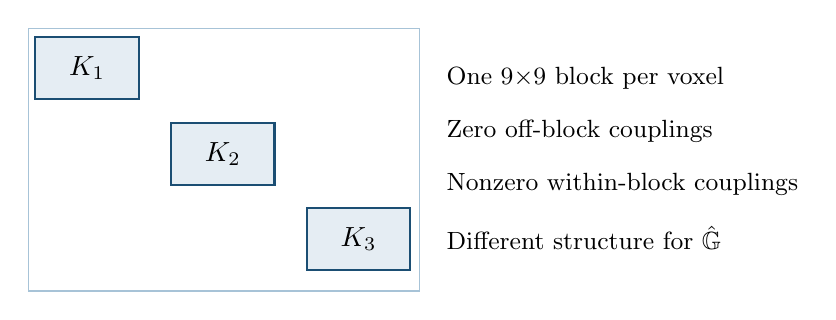
\begin{tikzpicture}[scale=.75]
 \foreach \a/\label in {0/$K_1$,1/$K_2$,2/$K_3$}{
   \fill[blue!12] (\a*2.3,-\a*1.45) rectangle ++(1.75,-1.05);
   \draw[blue!75!black,thick] (\a*2.3,-\a*1.45) rectangle ++(1.75,-1.05);
   \node at (\a*2.3+.875,-\a*1.45-.525) {\label};
 }
 \draw[blue!40] (-.12,.15) rectangle (6.5,-4.3);
 \node[anchor=west,font=\small] at (6.8,-.7) {One 9$\times$9 block per voxel};
 \node[anchor=west,font=\small] at (6.8,-1.6) {Zero off-block couplings};
 \node[anchor=west,font=\small] at (6.8,-2.5) {Nonzero within-block couplings};
 \node[anchor=west,font=\small] at (6.8,-3.4) {Different structure for $\hat{\Gop}$};
\end{tikzpicture}
\end{center}
\begin{caution}
Although the tangent is local, \emph{the equilibrium solve is not local}. The full physical-space action involves $\Gop$, which couples the entire periodic cell. Likewise, FFT's frequency-wise independent projection does not decouple a heterogeneous nonlinear constitutive problem: spatial multiplication by the varying $\Kop(\Xvec)$ couples Fourier modes.
\end{caution}

\clearpage
\section{Newton--CG--FFT algorithm and comparison with FEM}
\subsection{Nested solver flowchart}
The paper's Section 2 derives the linear system; Section 3 describes the load-increment implementation and CG solve. The chart below is an explanatory consolidation of those descriptions (the detailed first-iteration load treatment is beyond Eq. (24)).
\begin{center}
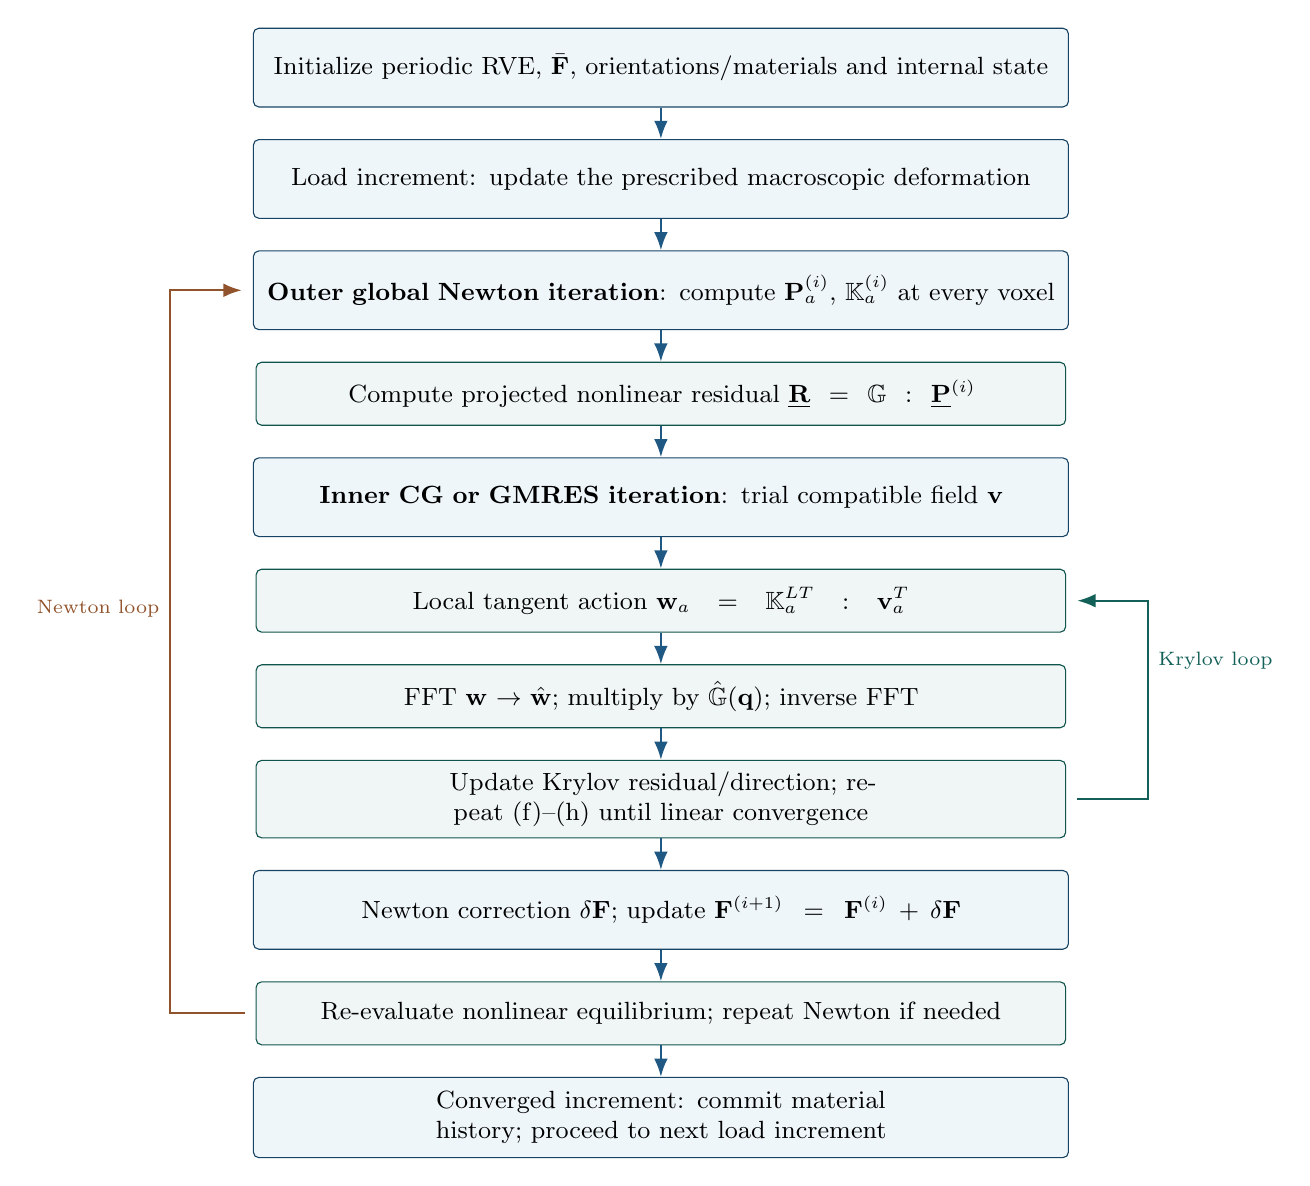
\begin{tikzpicture}[node distance=4mm]
\node[flow] (a) {Initialize periodic RVE, $\bar\F$, orientations/materials and internal state};
\node[flow,below=of a] (b) {Load increment: update the prescribed macroscopic deformation};
\node[flow,below=of b] (c) {\textbf{Outer global Newton iteration}: compute $\Pstress_a^{(i)}$, $\Kop_a^{(i)}$ at every voxel};
\node[minor,below=of c] (d) {Compute projected nonlinear residual $\underline{\mathbf R}=\Gop:\underline\Pstress^{(i)}$};
\node[flow,below=of d] (e) {\textbf{Inner CG or GMRES iteration}: trial compatible field $\mathbf v$};
\node[minor,below=of e] (f) {Local tangent action $\mathbf w_a=\Kop_a^{LT}:\mathbf v_a^T$};
\node[minor,below=of f] (g) {FFT $\mathbf w$ $\to$ $\hat{\mathbf w}$; multiply by $\hat\Gop(\mathbf q)$; inverse FFT};
\node[minor,below=of g] (h) {Update Krylov residual/direction; repeat (f)--(h) until linear convergence};
\node[flow,below=of h] (i) {Newton correction $\delta\F$; update $\F^{(i+1)}=\F^{(i)}+\delta\F$};
\node[minor,below=of i] (j) {Re-evaluate nonlinear equilibrium; repeat Newton if needed};
\node[flow,below=of j] (k) {Converged increment: commit material history; proceed to next load increment};
\foreach \u/\v in {a/b,b/c,c/d,d/e,e/f,f/g,g/h,h/i,i/j,j/k}{\draw[arr] (\u)--(\v);}
\draw[arr,teal!80!black] ([xshift=4pt]h.east) -- ++(.9,0) |- ([xshift=4pt]f.east) node[pos=.35,right,font=\scriptsize] {Krylov loop};
\draw[arr,warm!90!black] ([xshift=-4pt]j.west) -- ++(-.95,0) |- ([xshift=-4pt]c.west) node[pos=.28,left,font=\scriptsize] {Newton loop};
\end{tikzpicture}
\end{center}
During an inner Krylov solve, $\Kop^{(i)}$ is the fixed linearization of the current Newton state; FFT/IFFT is applied repeatedly to different search-direction fields. At the next Newton step, new stresses and tangents are computed. For inelastic models, local constitutive Newton iterations may add a fourth nested layer (inside each voxel), distinct from the global equilibrium Newton solver.

\subsection{Side-by-side with finite-element mechanics}
\begin{center}\small
\begin{tabularx}{\textwidth}{@{}lXX@{}}\toprule
Aspect & Displacement-based finite elements & Variational FFT in source\\\midrule
Primary field & Nodal displacement $\uve_a$ & Grid deformation-gradient $\F_a$\\
Interpolation & Piecewise polynomial; local supports & Trigonometric cardinal; global support\\
Compatibility & $\F=\mathbf I+\nabla\uve$ by construction & Projection onto compatible gradient fluctuations\\
Constitutive response & Local at FE quadrature points & Local at voxel/grid nodes\\
Global residual & Assembled weak-form force imbalance & $\Gop:\Pstress$ projected field\\
Newton tangent & FE Jacobian assembled or matrix-free & Local tangent plus global FFT projector\\
Linear algebra & Direct or Krylov methods & Matrix-free Krylov method (CG in paper)\\
Global equilibrium & Yes & Yes\\\bottomrule
\end{tabularx}
\end{center}

\section{Appendix D: Proof of the projection operator --- Equations (50)--(55)}
Appendix D proves why Eq. (19) is a \emph{compatibility projector}, rather than simply introducing it as an ad hoc global coupling. It reduces the fourth-order tensor projection to a vector projection for every row, checks that all projected rows are curl-free, and finally checks that already compatible zero-mean fields are unchanged.

\subsection{Factor the fourth-order tensor into a row-wise projector (D50)}
The authors rewrite Eq. (19) as
\begin{equation}
\hat G_{ijlm}(\mathbf q)=\delta_{im}\hat g_{jl}(\mathbf q),\qquad
\hat{\mathbf g}(\mathbf q)=
\begin{cases}\mathbf0,&\mathbf q=\zero,\\[3pt]
\displaystyle\frac{\bm\xi\otimes\bm\xi}{|\bm\xi|^2},&\mathbf q\neq\zero.
\end{cases}
\Dtag{50}\label{pd50}\end{equation}
For nonzero frequency, this is the ordinary projection matrix onto the direction of $\bm\xi$:
\[
\hat{\mathbf a}=\hat{\mathbf g}\,\hat{\mathbf b}
=\frac{\bm\xi(\bm\xi\cdot\hat{\mathbf b})}{|\bm\xi|^2}.
\]
In 2D with $\bm\xi=(1,1)^T$, the matrix is $\hat{\mathbf g}=\tfrac12\left[\begin{smallmatrix}1&1\\1&1\end{smallmatrix}\right]$. Acting on $\hat{\mathbf b}=(2,0)^T$ returns $(1,1)^T$, which is parallel to $\bm\xi$.

\subsection{Project every row of an arbitrary tensor (D51)--(D52)}
For $\mathbf A=\Gop*\mathbf B$, convolution gives
\begin{equation}
\hat A_{ij}(\mathbf q)
=\hat G_{ijlm}(\mathbf q)\hat B_{ml}(\mathbf q)
=\delta_{im}\hat g_{jl}(\mathbf q)\hat B_{ml}(\mathbf q).
\Dtag{51}\label{pd51}\end{equation}
Using $\delta_{im}$ leaves $\hat A_{ij}=\hat g_{jl}\hat B_{il}$. Thus one may focus on any row of $\mathbf B$: call it $\mathbf b$. Its projected row is
\begin{equation}
\mathbf a=\mathbf g*\mathbf b.
\Dtag{52}\label{pd52}\end{equation}
This reduces tensor-gradient compatibility to the familiar curl-free property of a vector field.

\subsection{First part of the proof: every projected field is compatible (D53)}
For $\mathbf q\neq\zero$, the projected Fourier coefficient is parallel to the wavevector:
\[
\hat{\mathbf a}(\mathbf q)=\frac{\bm\xi\big(\bm\xi\cdot\hat{\mathbf b}\big)}{|\bm\xi|^2}.
\]
The physical curl becomes multiplication by $i2\pi\bm\xi\times$ in Fourier space. Omitting this harmless common nonzero scalar in the test of vanishing curl, the paper uses
\begin{equation}
\bm\xi\times\hat{\mathbf a}(\mathbf q)
=\begin{cases}
\zero,&\mathbf q=\zero,\\[3pt]
\displaystyle\frac{\big(\bm\xi\times\bm\xi\big)
\big(\bm\xi\cdot\hat{\mathbf b}\big)}{|\bm\xi|^2}=\zero,&\mathbf q\ne\zero.
\end{cases}
\Dtag{53}\label{pd53}\end{equation}
Since $\bm\xi\times\bm\xi=\zero$, the projected vector field is curl-free. On a periodic cell, the zero-mean condition rules out a nonzero constant harmonic component and makes it a periodic scalar gradient. Since this argument applies separately to each tensor row, $\mathbf A$ is a compatible tensor field.

\subsection{Second part: all compatible zero-mean fields are retained (D54)--(D55)}
Let the row field $\mathbf b$ already be compatible, i.e. $\mathbf b=\nabla_0 f$ for a periodic scalar $f$. In Fourier space its coefficient is $\hat{\mathbf b}=i2\pi\bm\xi\hat f$. The paper absorbs the common $i2\pi$ into the scalar coefficient for the projection calculation, writing $\hat{\mathbf b}=\bm\xi\hat f$ in that abbreviated convention. Then
\begin{equation}
\hat{\mathbf g}\,\hat{\mathbf b}=
\begin{cases}
\zero,&\mathbf q=\zero,\\[3pt]
\displaystyle\frac{\bm\xi(\bm\xi\cdot\bm\xi)\hat f}{|\bm\xi|^2},&\mathbf q\ne\zero.
\end{cases}
\Dtag{54}\label{pd54}\end{equation}
For nonzero modes the numerator factor cancels the denominator, yielding
\begin{equation}
\boxed{\hat{\mathbf g}\,\hat{\mathbf b}=\bm\xi\hat f=\hat{\mathbf b}.}
\Dtag{55}\label{pd55}\end{equation}
The compatible zero-mean field is unchanged: there are no compatible gradient fluctuations excluded from the projector's range.

\subsection{Additional consequences: symmetry, idempotence and equilibrium}
The matrix $\hat{\mathbf g}=\bm\xi\bm\xi^T/|\bm\xi|^2$ obeys
\[
\hat{\mathbf g}^T=\hat{\mathbf g},\qquad
\hat{\mathbf g}^{\,2}=\hat{\mathbf g},
\]
so it is an \emph{orthogonal projector} in the relevant Fourier vector space. On the projected deformation-gradient space, this means that applying it twice is no different from applying it once. In contrast, when applied to stress and the result is set to zero, it imposes the divergence-free condition: a stress equilibrated against every compatible periodic virtual gradient belongs to the \emph{orthogonal complement} of that gradient space. The average stress is unrestricted.

\section{Crystal-plasticity interpretation and practical implementation notes}
For a conventional local finite-strain crystal plasticity or dislocation-density crystal plasticity (DDCP) material model, a voxel-local trial update may be represented schematically by
\[
(\F_a,\bm\alpha_a^{\mathrm{old}},\Delta t,\text{orientation}_a)
\longmapsto
(\Pstress_a,\Kop_a^{\mathrm{alg}},\bm\alpha_a^{\mathrm{trial}}).
\]
The full Newton--Krylov solver needs the \emph{correct stress measure and algorithmic tangent} consistent with the paper's total-reference formulation. If a CP material routine returns Cauchy stress $\bm\sigma$ or Kirchhoff stress $\bm\tau=J\bm\sigma$, the PK1 stress is $\Pstress=\bm\tau\F^{-T}=J\bm\sigma\F^{-T}$; the tangent requires corresponding product-rule and geometric terms, not just a relabeling of components. Since Eqs. (1)--(24) are derived for an elastic law, this adaptation is a constitutive implementation extension rather than a derivation asserted within Section 2.

History-dependent models require consistent \emph{trial versus committed} internal states: global Newton residual evaluations should not irreversibly commit slip or dislocation density before the load increment has converged. If the projected tangent becomes nonsymmetric, loses positive definiteness, or the material response softens, using standard CG without verifying its assumptions can fail; GMRES or suitable alternatives/preconditioning should be considered. Compatibility and prescribed mean deformation are separate numerical requirements and must not be lost through the choice of linear solver or initialization.

\section{Consolidated mathematical roadmap}
\begin{center}\small
\begin{longtable}{@{}p{.12\textwidth}p{.33\textwidth}p{.47\textwidth}@{}}\toprule
Paper Eq. & Principal mathematical statement & Interpretation\\\midrule\endhead
(1)--(2) & $\nabla_0\cdot\Pstress^T=0$, $\Pstress=\Pstress(\F)$ & Nonlinear finite-strain mechanical equilibrium\\
(3)--(4) & Weak form and integration by parts & Periodic virtual work; boundary term cancels\\
(5) & $\int\delta\F:\Pstress^T=0$ & Use compatible variations of deformation gradient\\
(6)--(7) & Project arbitrary test tensors & Insert compatibility into weak form via symmetric projector\\
(8)--(11) & Trigonometric cardinal interpolation & Global basis, local stored nodal values\\
(12)--(14) & Discrete weak form and trapezoidal quadrature & Projected residual at all collocation nodes\\
(15)--(16) & $\IFFT\{\hat\Gop:\FT(\Pstress)\}=0$ & Fast global equilibrium-residual evaluation\\
(17) & $\Pstress_a(\F_a)$ & Voxel-local constitutive updates\\
(18)--(19) & Fourier block diagonal; $\hat G_{ijlm}$ & Frequency-wise geometric projector, independent of stiffness\\
(20) & Mean of projected field is zero & Independent control of imposed macroscopic deformation\\
(21)--(22) & Newton correction; local tangent & Linearize constitutive response at present iterate\\
(23)--(24) & $\Gop:\Kop^{LT}:\delta\F^T=-\Gop:\Pstress$ & Globally coupled Newton correction with block-local tangents\\
(D50)--(D55) & Projection onto $\bm\xi$, curl-free and unchanged gradient & Formal proof of complete zero-mean compatibility projector\\\bottomrule
\end{longtable}
\end{center}

\begin{insight}
\textbf{Final conceptual formula:}\par\medskip
\centering
$\displaystyle
\underbrace{\delta\F}_{\substack{\text{unknown compatible}\\\text{global correction}}}
\xrightarrow{\quad\Kop\quad}
\underbrace{\delta\Pstress}_{\substack{\text{local constitutive}\\\text{stress correction}}}
\xrightarrow{\quad\Gop\ \mathrm{via\ FFT}\quad}
\underbrace{\delta\mathbf R}_{\substack{\text{global projected}\\\text{equilibrium correction}}}.$
\par\medskip
\raggedright
The linearized \emph{global} Newton system is solved iteratively, even though stress and tangent are evaluated \emph{locally} and no complete global stiffness matrix is assembled.
\end{insight}

\begin{thebibliography}{9}
\bibitem{degeus2017} T. W. J. de Geus, J. Vond\v{r}ejc, J. Zeman, R. H. J. Peerlings, and M. G. D. Geers, ``Finite strain FFT-based non-linear solvers made simple,'' \emph{Computer Methods in Applied Mechanics and Engineering}, vol. 318, pp. 412--430, 2017. \href{https://doi.org/10.1016/j.cma.2016.12.032}{doi:10.1016/j.cma.2016.12.032}; \href{https://arxiv.org/abs/1603.08893}{arXiv:1603.08893v3}. Source for all tagged paper equations.
\bibitem{moulinec1998} H. Moulinec and P. Suquet, ``A numerical method for computing the overall response of nonlinear composites with complex microstructure,'' \emph{Computer Methods in Applied Mechanics and Engineering}, vol. 157, pp. 69--94, 1998. Cited in the source paper for the reference-medium FFT approach.
\end{thebibliography}
\end{document}
